\documentclass[../../main]{subfiles}

\renewcommand\thesection{\arabic{section}}


\begin{document}

\section{Structural Frame} \label{sec:}

The structural frame of the incubator carries all the weight of the rest of the
systems. And provides mounting points for the different parts\footnote{like
exhaust pipes, hatches etc} of the other systems. So it is important for it to
be strong and lasting. Although it was preferable to use aluminum, because of
the manufacturing difficulties\footnote{namely cutting and welding}, we have
resorted to \emph{plywood}. Figure \ref{fig:frameCAD} shows the CAD rendering
of the frame.

\begin{figure}
    \centering
    \hspace{1cm}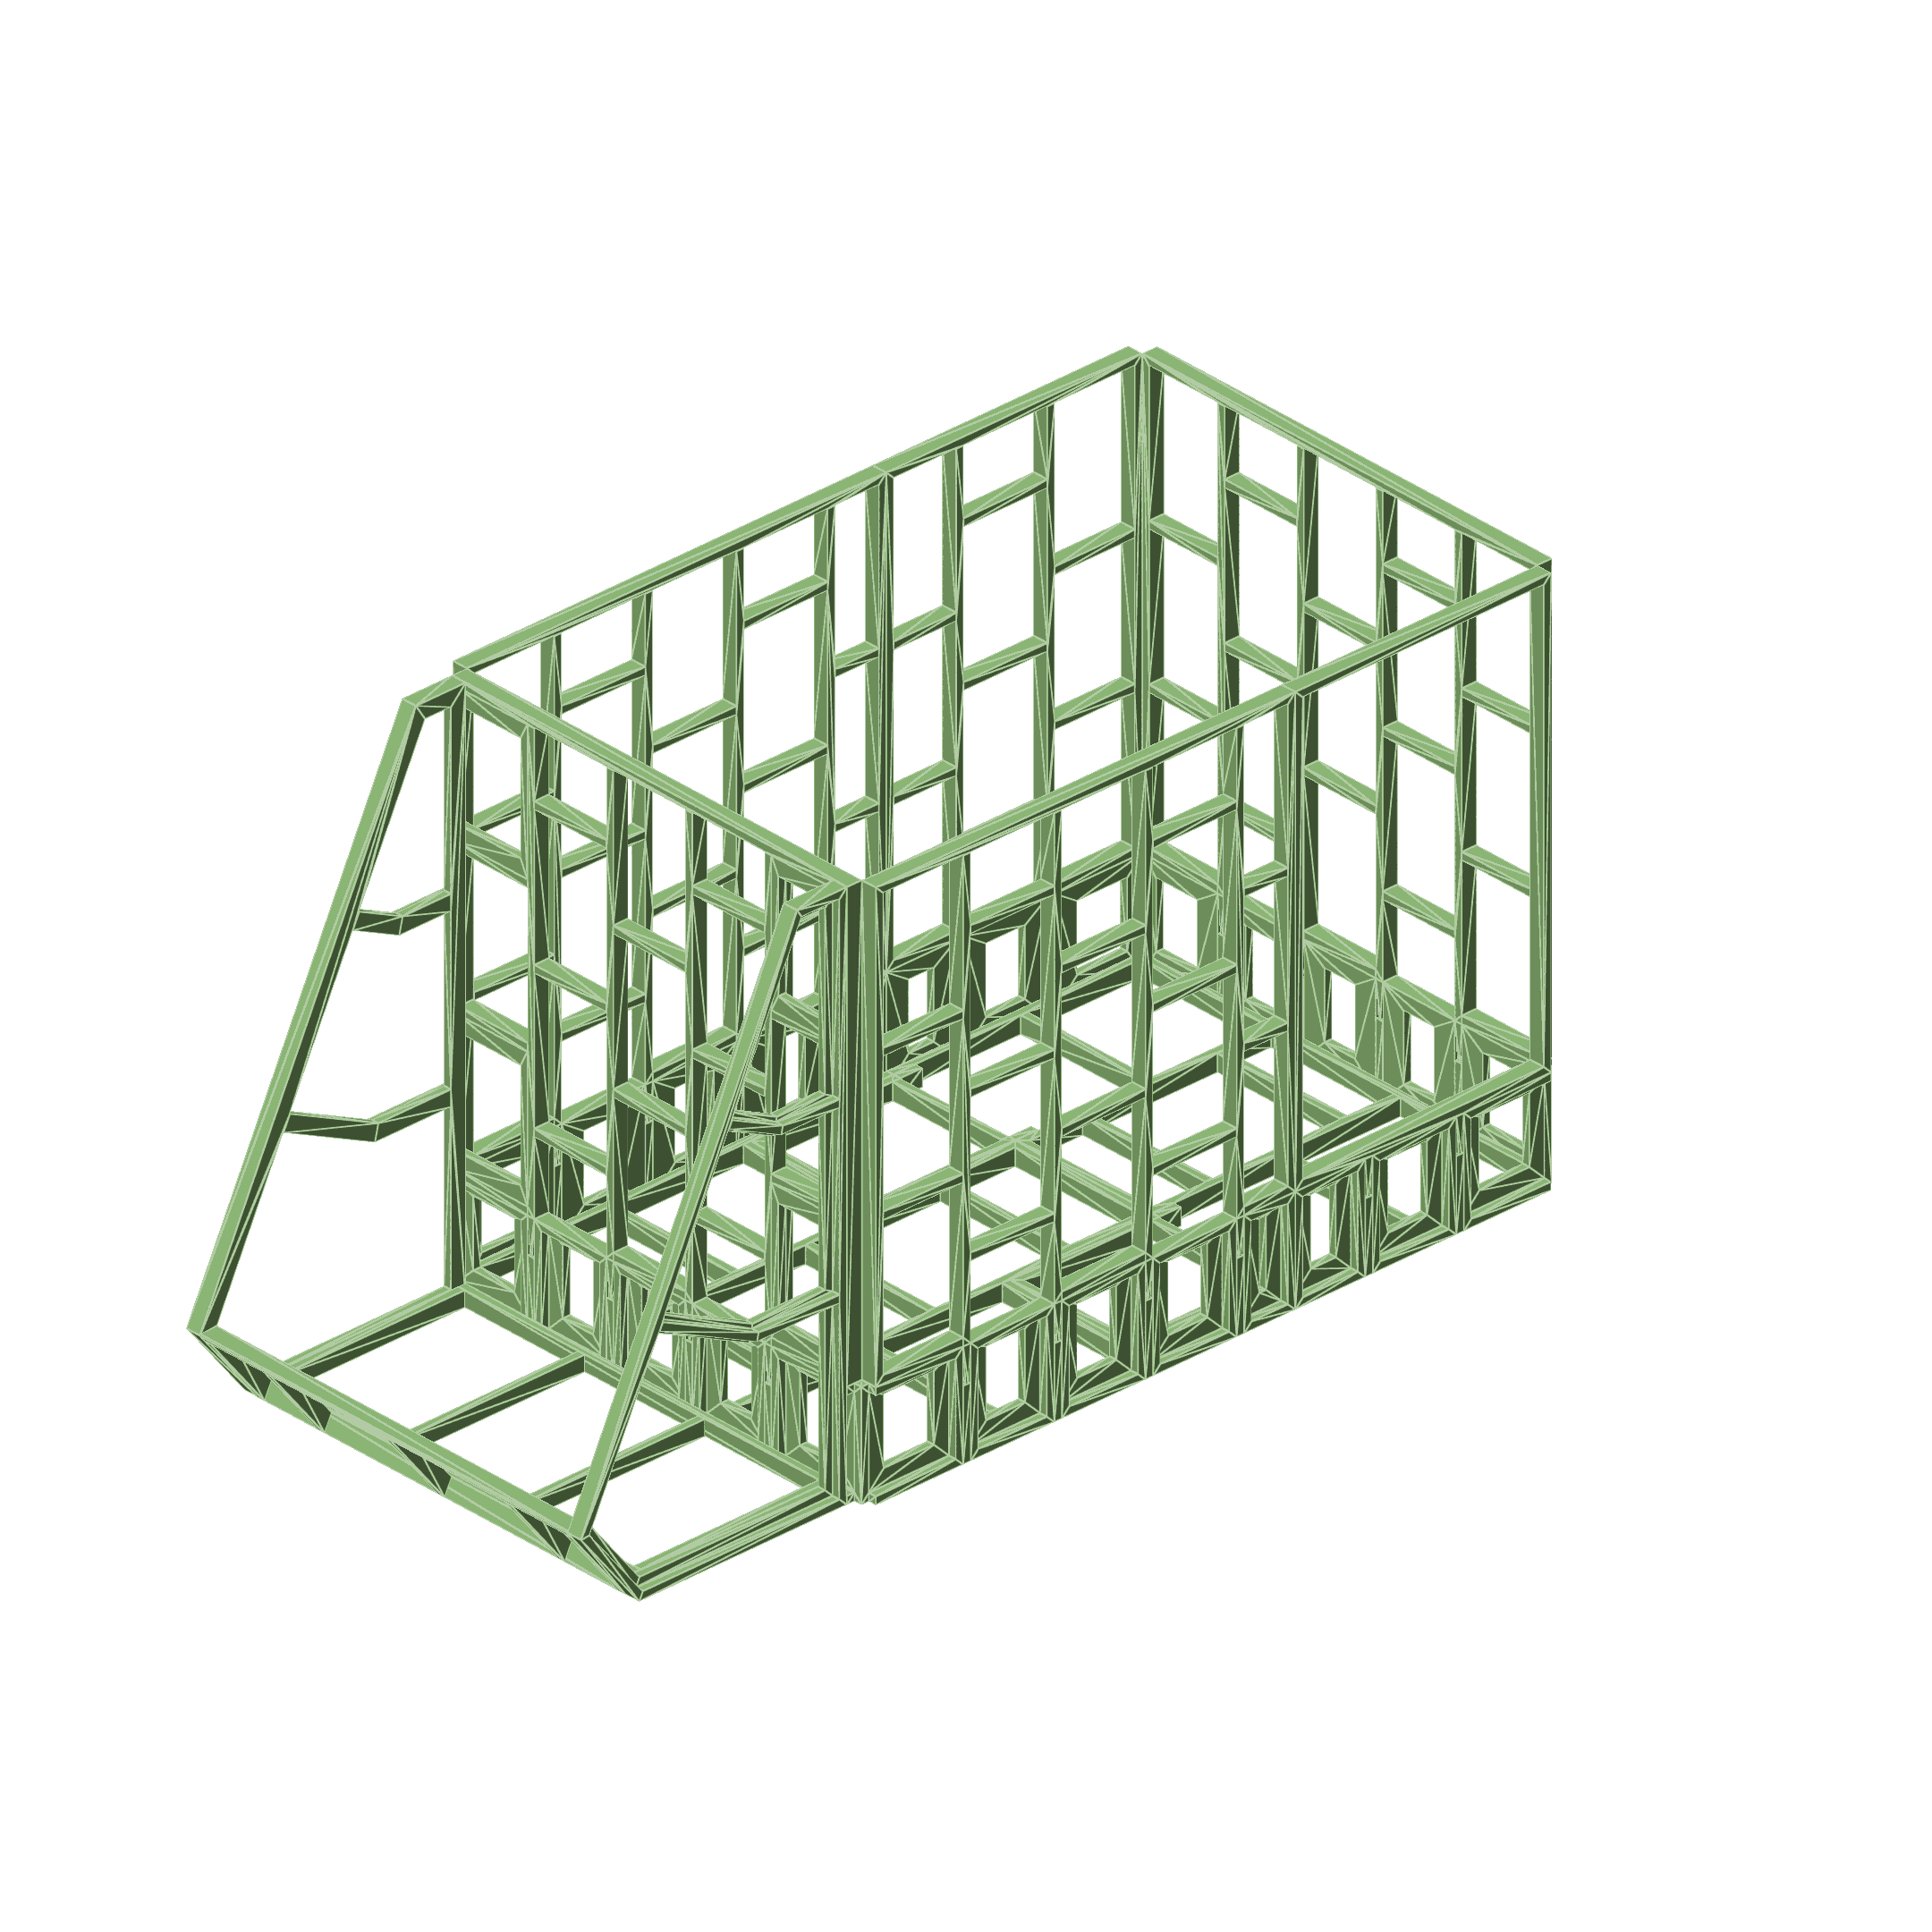
\includegraphics [
        height = 0.5\textwidth,
        max width = \IGXMaxWidth,
        max height = \IGXMaxHeight,
        \IGXDefaultOptionalArgs,
        trim = {7cm 11cm 7cm 11cm},
        clip,
    ] {pics/frame_cad.png}
    \captionof{figure} {Assembled CAD rendering of the structural frame.}
    \label{fig:frameCAD}
\end{figure}

A plywood based frame is easier to build, but it would be heavy and becomes
expensive if we decide to directly build the frame using plywood sheets.
Inorder to address this issue, we have decided to use $1.8\si{cm}$ and
$2\si{cm}$ plywood strips to build the frame. This would massively reduce the
amount of plywood needed for the support frame. By providing hatch support
frames, we can compensate for the structural rigidity that we would lose by
using this method. Also the entire structural frame is further divided into
different segments for the sake of transportation. And these segments can be
dis-assembled and assembled before and after transportation using nuts and
bolts.

\alertNote{
    Figure \ref{fig:frameCAD} and table \ref{tbl:frameSegments} are only shows
    the frame for the \emph{electronics bay} and the \emph{incubator area}. The
    CAD design for the \emph{water} and \emph{fertilizer reservoir} are still
    in progress. They will be at the back side of the incubator area frame.
}

\begin{center}

    \begin{tabularx} {\textwidth} {
            >{\centering \arraybackslash}X
            >{\centering \arraybackslash}X
            >{\centering \arraybackslash}X
        }

        \toprule

        Electronics Bay & Front Base & Back Base \\ \midrule

        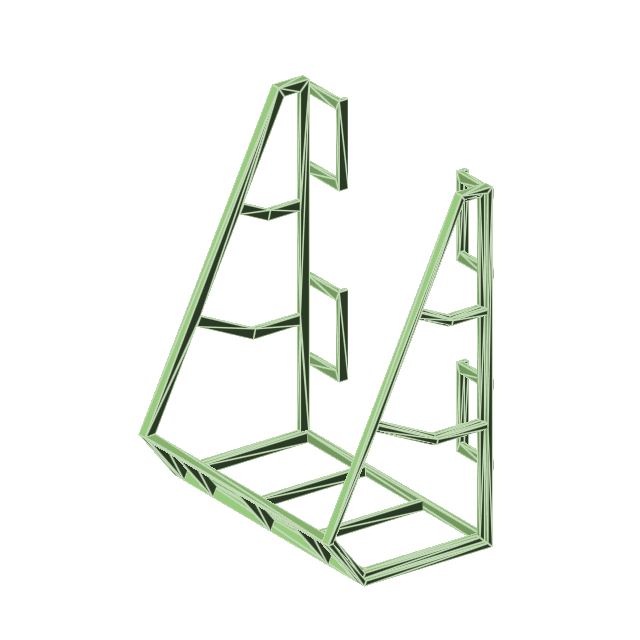
\includegraphics [
            width = 0.3\textwidth,
        ] {pics/elec_bay.png}

        &

        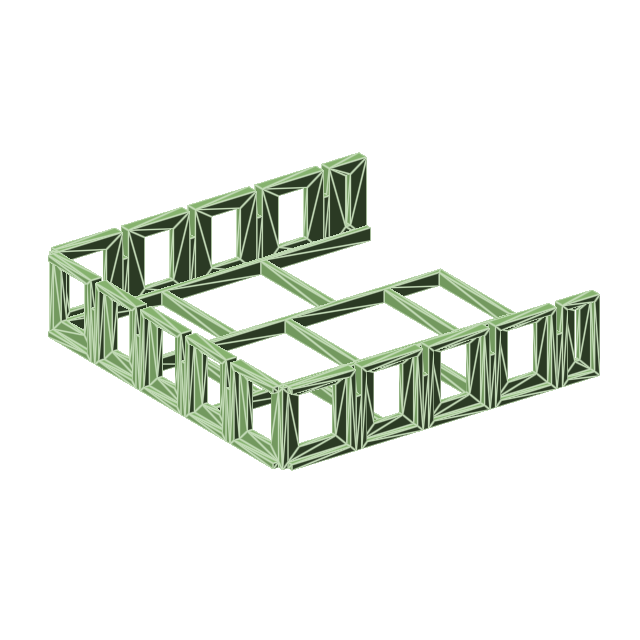
\includegraphics [
            width = 0.3\textwidth,
        ] {pics/front_base.png}

        &

        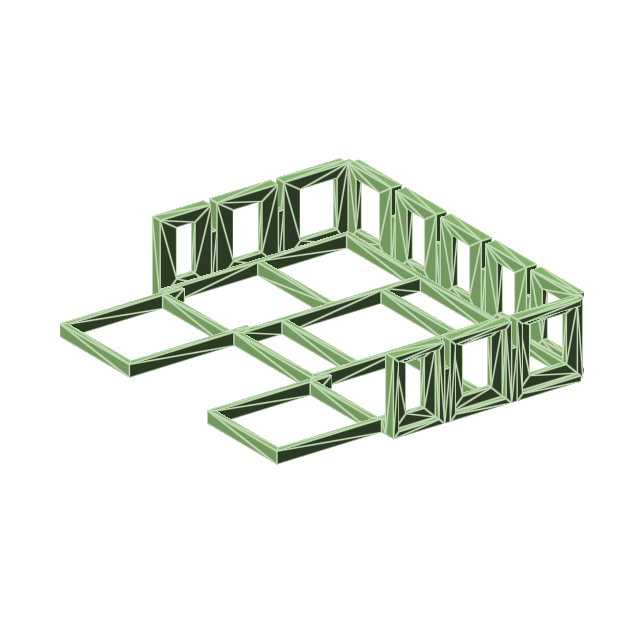
\includegraphics [
            width = 0.3\textwidth,
        ] {pics/back_base.png}

        \\ \midrule

        Front Side Panels & Back Side Panels & Front and Back Panels \\ \midrule

        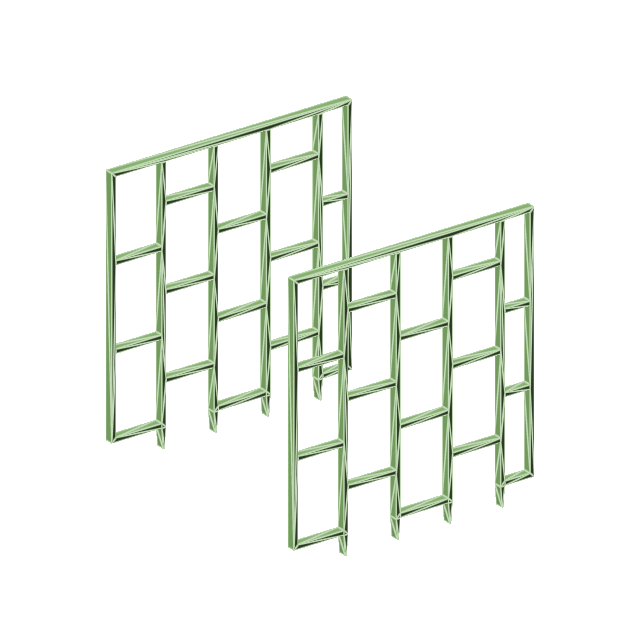
\includegraphics [
            width = 0.3\textwidth,
        ] {pics/front_side_panels.png}

        &

        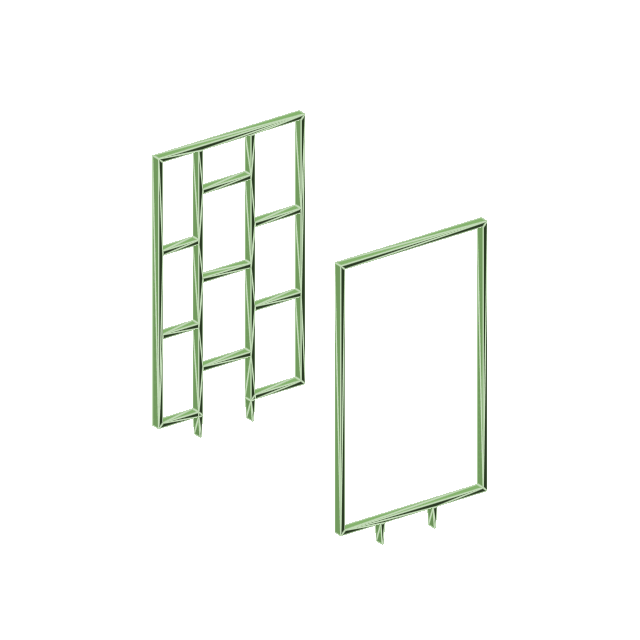
\includegraphics [
            width = 0.3\textwidth,
        ] {pics/back_side_panels.png}

        &

        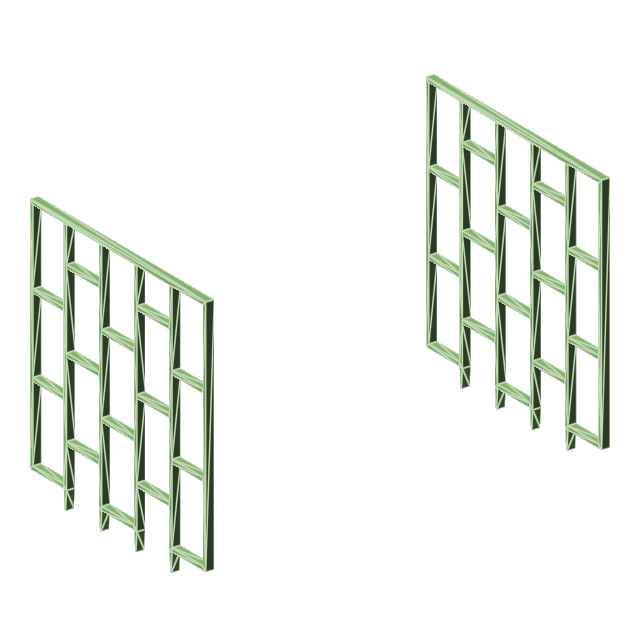
\includegraphics [
            width = 0.3\textwidth,
        ] {pics/front_back_panels.png}

        \\

        \bottomrule

    \end{tabularx}

    \captionof{table}{Different segments of the incubator structural frame.}
    \label{tbl:frameSegments}

\end{center}

\subsection{Progress So Far}

At the moment the front base and back base are build. Please ref figures \ref{fig:frontBackBase} and
\ref{fig:frontBackDisBase} for the front and back bases that we have build.

\alertImportant{
    It is important to leave clearance spaces while designing parts that slides or attaches
    together. And important to account for the thickness variation with the plywood, if you
    are trying to build anything with plywood. In our case, ignorance on that part caused
    different parts to not fit properly and required additional sanding and cutting for them
    to fit properly.
}

\begin{center}
    \begin{minipage} {0.45\textwidth}
        \begin{figure}
            \centering
            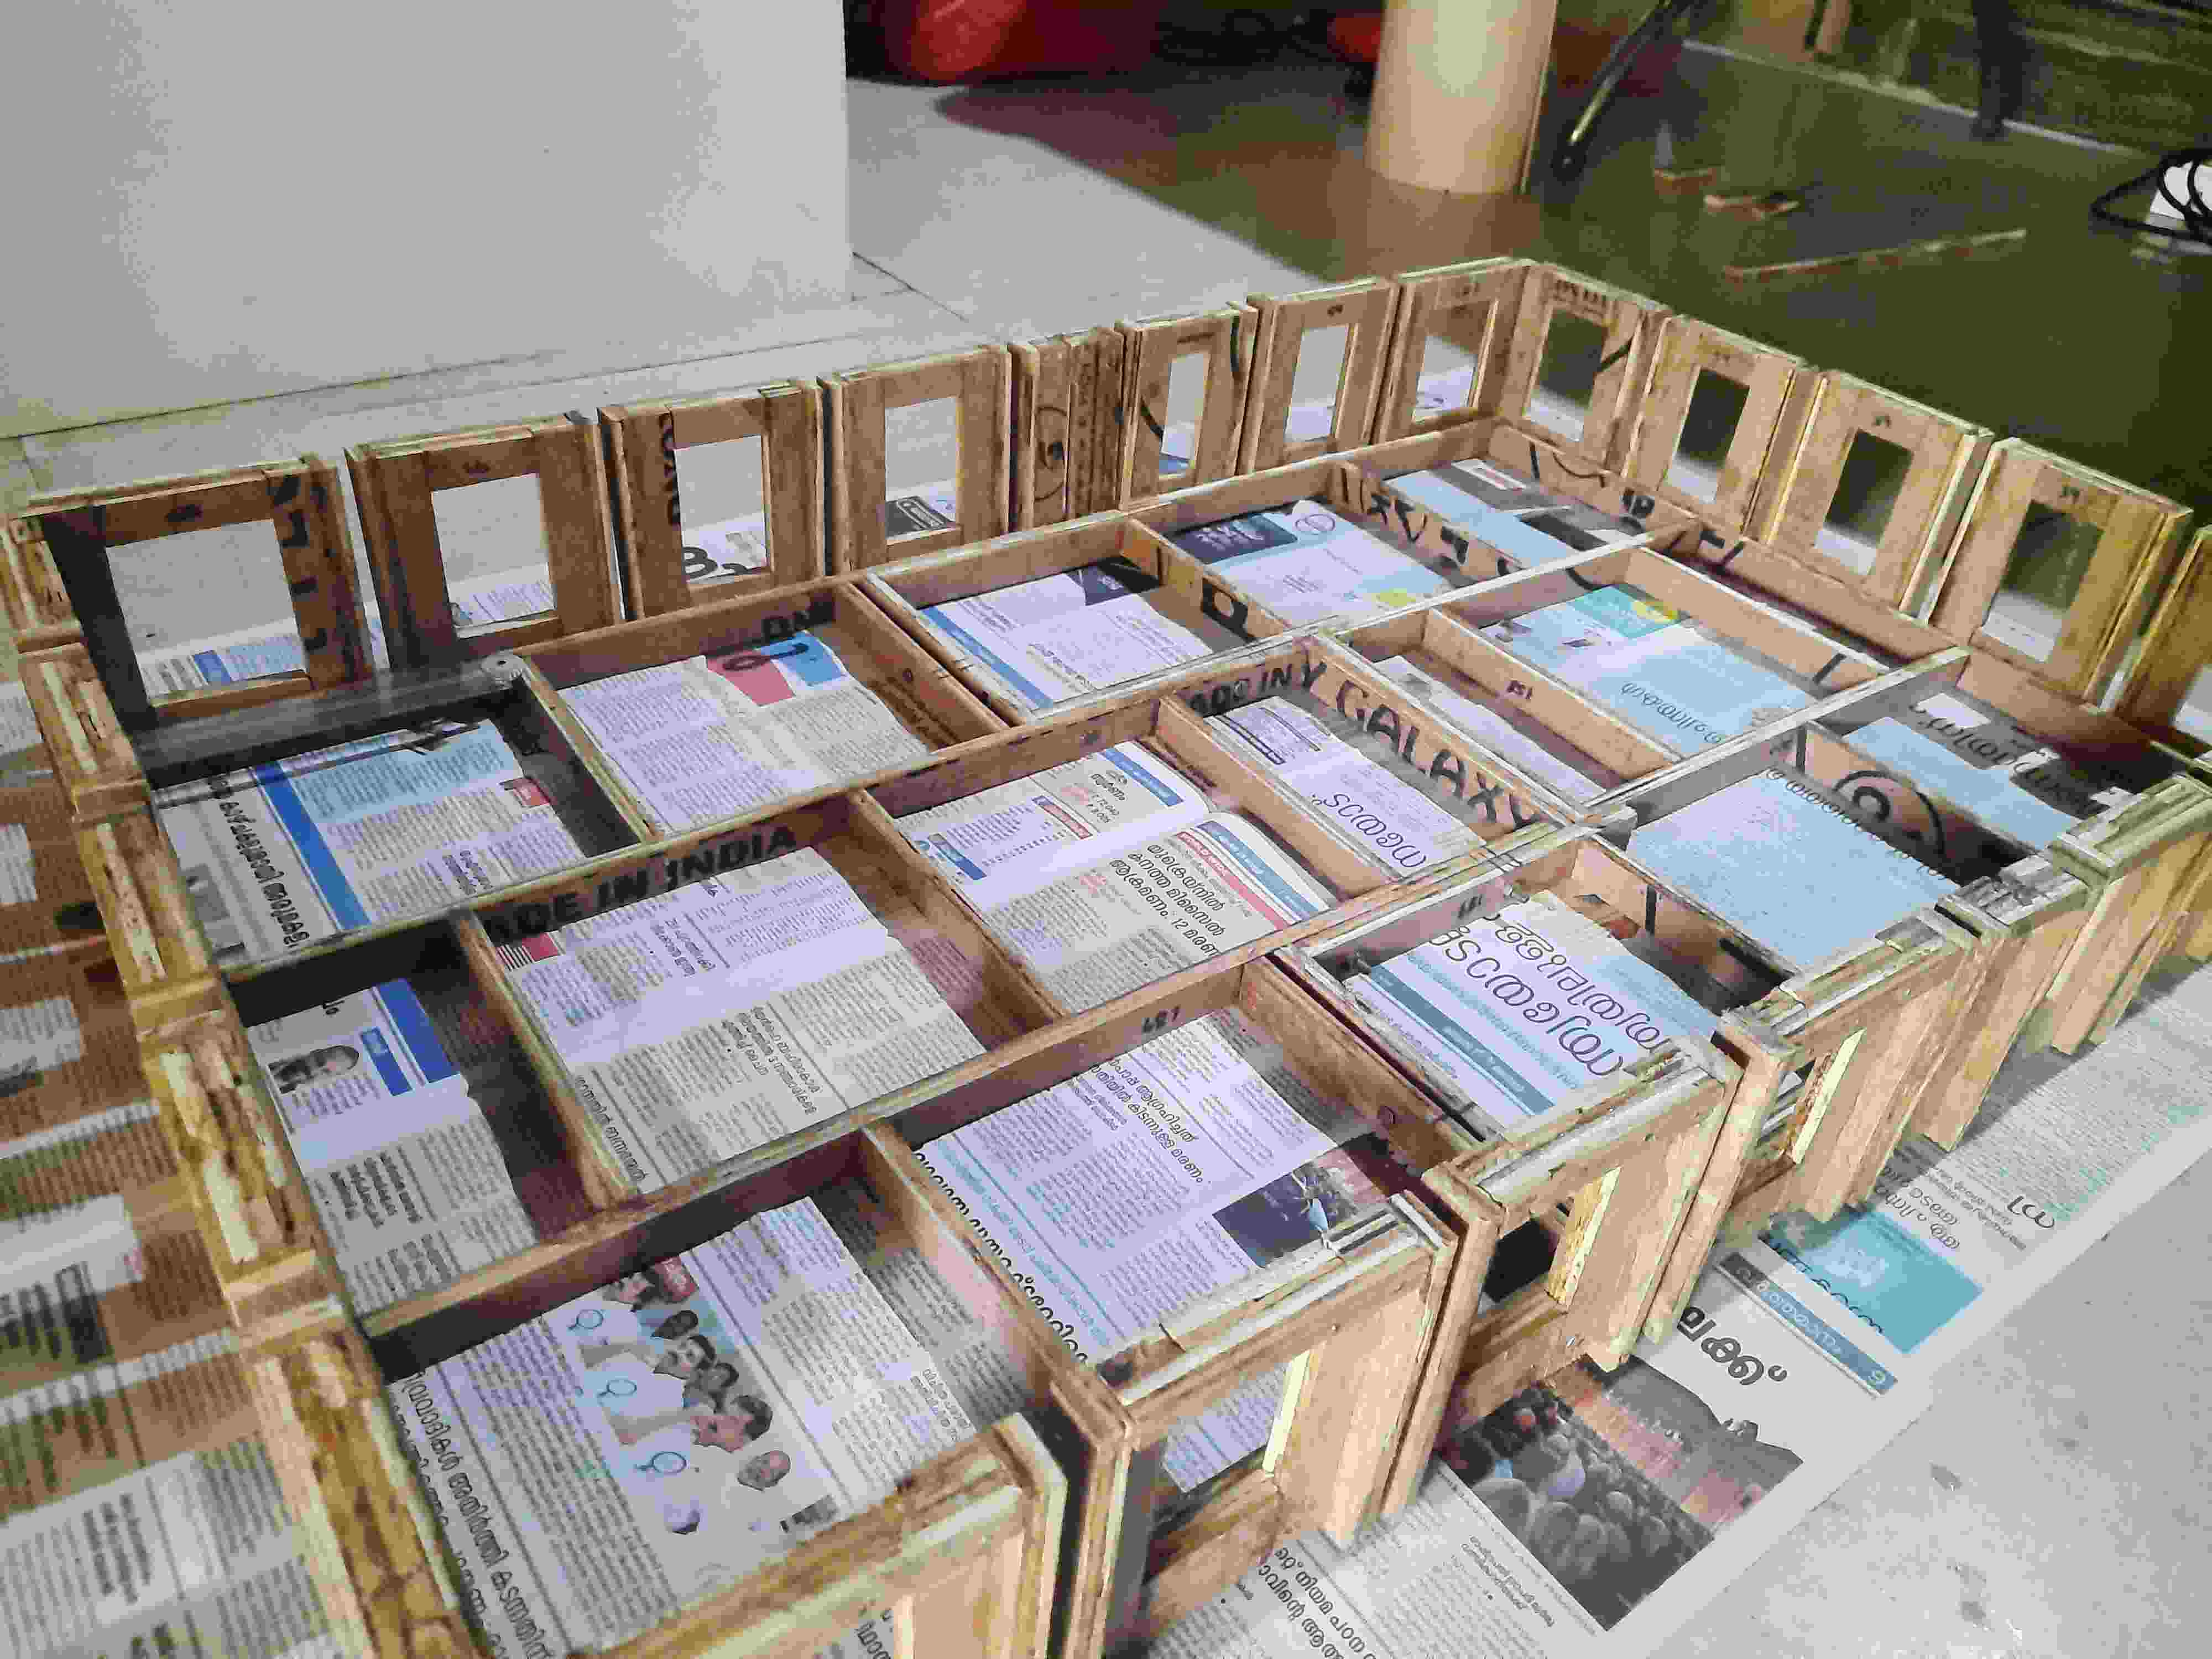
\includegraphics [
                height = 0.225\textheight,
                max width = \IGXMaxWidth,
                max height = \IGXMaxHeight,
                \IGXDefaultOptionalArgs,
            ] {pics/base_attached.jpg}
            \captionof{figure} {Front and back bases attached together using nuts and bolts.}
            \label{fig:frontBackBase}
        \end{figure}
    \end{minipage}
    \hfill
    \begin{minipage} {0.45\textwidth}
        \begin{figure}
            \centering
            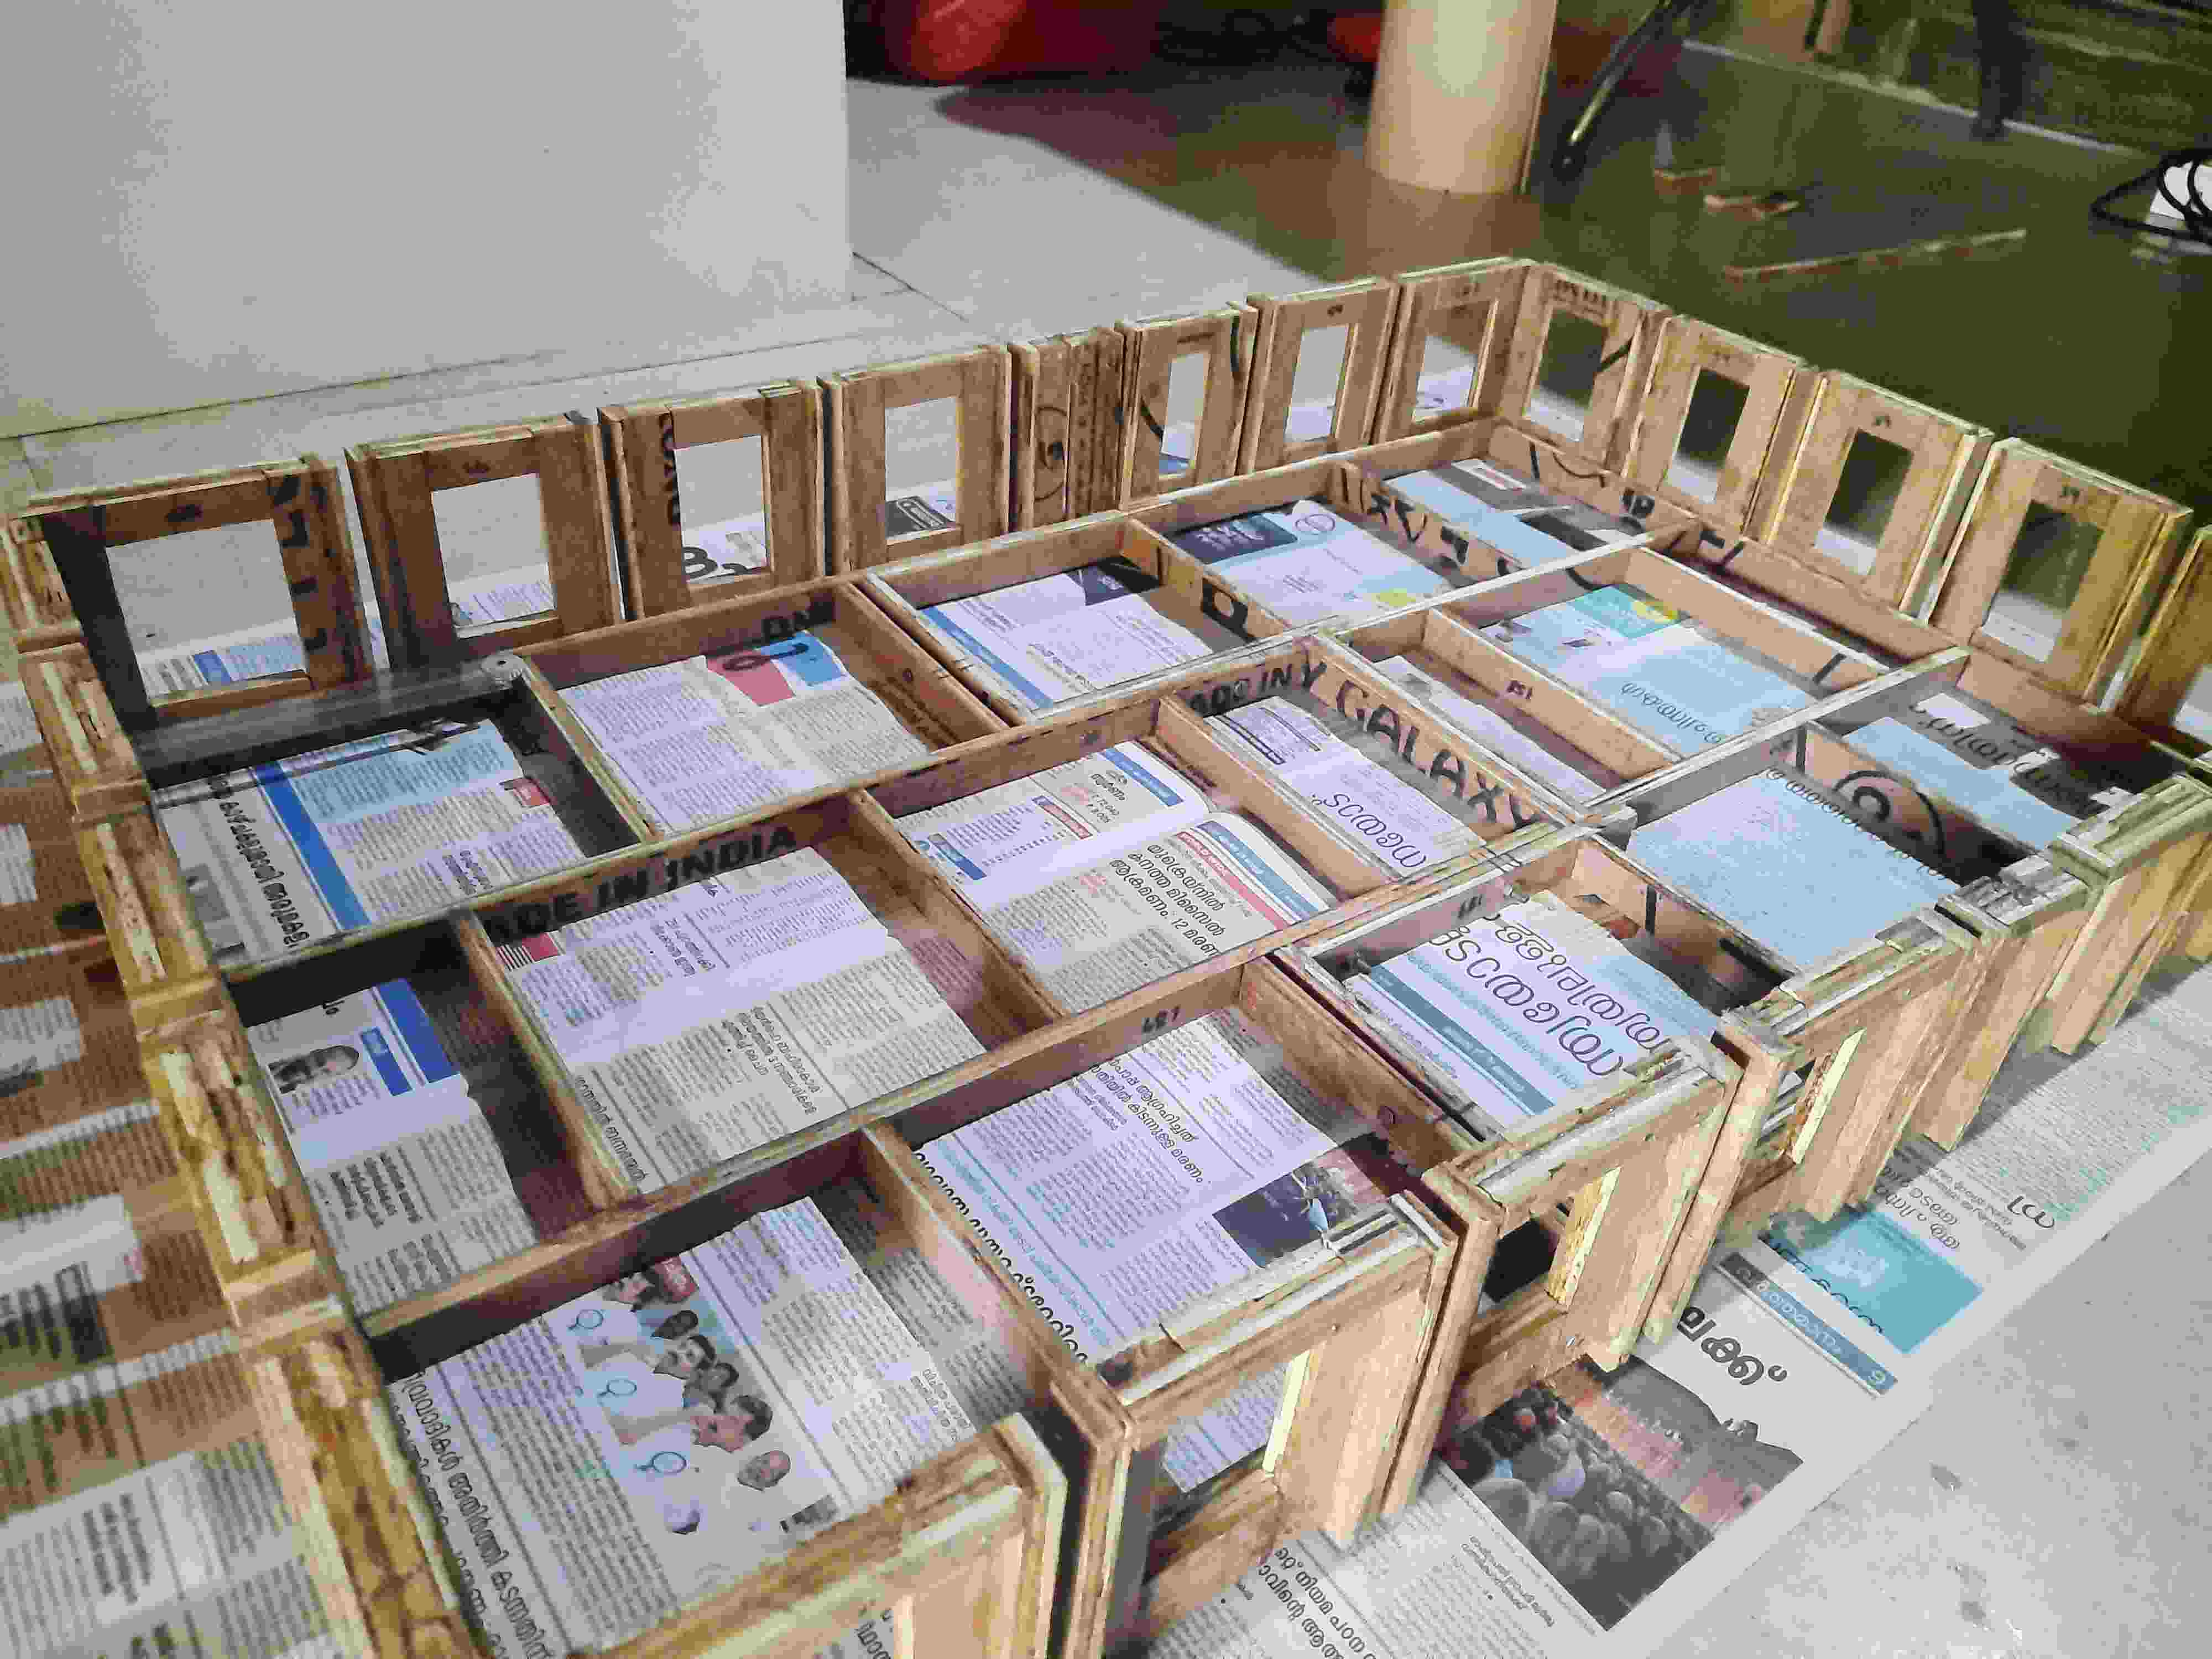
\includegraphics [
                height = 0.225\textheight,
                max width = \IGXMaxWidth,
                max height = \IGXMaxHeight,
                \IGXDefaultOptionalArgs,
            ] {pics/base_attached.jpg}
            \captionof{figure} {Dis-assembled front and back bases.}
            \label{fig:frontBackDisBase}
        \end{figure}
    \end{minipage}
\end{center}

% back_base.png
% back_side_hatch.png
% back_side_panel.png
% elec_bay.png
% front_base.png
% front_panel.png
% front_side_panel.png

% back_base.png
% back_side_panels.png
% elec_bay.png
% front_back_panels.png
% front_base.png
% front_side_panels.png

\end{document}
